\begin{name}
	{\tenchude}
	{TOÁN 10}
	{LỚP TOÁN THẦY PHÁT}
	{Thời gian: 90 phút - Không kể thời gian phát đề}
\end{name}
\noindent{\bf\fontfamily{qag}\selectfont\color{violet}A. PHẦN TRẮC NGHIỆM}
\Opensolutionfile{ans}[ans/ans-0-GK1-CTST-De6-NH23-24]
%%==========Câu 1
\begin{ex}%[0D1Y1-1]
Trong các phát biểu sau, phát biểu nào là mệnh đề \textbf{đúng}?
\choice
{\True $\dfrac{1}{2}$ là số hữu tỉ}
{Hình bình hành có bốn cạnh bằng nhau}
{Tam giác có một góc bằng $60^{\circ}$ là tam giác đều}
{$6$ là số chính phương}
	\loigiai{
	}
\end{ex}

%%==========Câu 2
\begin{ex}%[0D1Y1-1]
	Trong các phát biểu sau, phát biểu nào là mệnh đề chứa biến?
	\choice
	{\True $2x+5>0$}
	{$\sqrt{2}$ là số hữu tỉ}
	{$5$ là số nguyên tố}
	{$8$ là hợp số}
	\loigiai{Chưa khẳng định được tính đúng sau của phát biểu \lq\lq $2x+5>0$\rq\rq. Khi cho $x$ một giá trị cụ thể mới khẳng định được tính đúng sai.
	}
\end{ex}

%%==========Câu 3
\begin{ex}%[0D1Y1-3]
Cho mệnh đề $P$: \lq\lq$\pi$ là một số vô tỉ\rq\rq. Mệnh đề nào sau đây là mệnh đề phủ định của $P$ ?
\choice
{$\pi$ là một số vô tỉ}
{\True $\pi$ không là một số vô tỉ}
{$\pi$ không là một số thực}
{$\pi$ không là một số hữu tỉ}
	\loigiai{
	}
\end{ex}

%%==========Câu 4
\begin{ex}%[0D1Y1-2]
Cho định lí $P \Rightarrow Q$. Phát biểu nào sau đây \textbf{đúng}?
	\choice
{$P$ là điều kiện cần để có $Q$}
{$Q$ là điều kiện đủ để có $P$}
{\True $P$ là điều kiện đủ để có $Q$}
{$Q$ là giả thiết của định lí}
	\loigiai{
	}
\end{ex}

%%==========Câu 5
\begin{ex}%[0D1Y1-4]
Đâu là mệnh đề đảo của mệnh đề: \lq\lq Nếu tam giác có hai cạnh bằng nhau thì tam giác đó là tam giác cân\rq\rq ?
\choice
{Một tam giác là tam giác cân nếu và chỉ nếu tam giác đó có 2 cạnh bằng nhau}
{Một tam giác không có hai cạnh bằng nhau thì tam giác đó không là tam giác cân}
{\True Nếu một tam giác là tam giác cân thì tam giác đó có hai cạnh bằng nhau}
{Tam giác đó là tam giác cân}
	\loigiai{
	}
\end{ex}

%%==========Câu 6
\begin{ex}%[0D1Y1-5]
Đâu là kí hiệu \lq\lq với mọi\rq\rq ?
	\choice
	{\True $\forall$}
	{$\in$}
	{$\exists$}
	{$\subset$}
	\loigiai{
	}
\end{ex}

%%==========Câu 7
\begin{ex}%[0D1Y2-1]
Cho tập hợp $A=\left\{x \in \mathbb{N}\,|\, x<4\right\}$. Tìm phát biểu \textbf{đúng}.
	\choice
	{\True $A=\left\{0;1;2;3\right\}$}
	{$A=\left\{1;2;3\right\}$}
	{$A=\left\{4\right\}$}
	{$A=\left\{0;1;2;3;4\right\}$}
	\loigiai{
	Vì $x<4$ và $x \in \mathbb{N}$ nên $x \in \left\{0;1;2;3\right\}$.\\
	Vậy $A=\left\{0;1;2;3\right\}$.
	}
\end{ex}

%%==========Câu 8
\begin{ex}%[0D1B2-2]
	Cho tập hợp $A=\left\{x \in \mathbb{N}\,|\, x-2\leq 0\right\}$. Số tập hợp con có hai phần tử của tập $A$ là
	\choice
	{$2$}
	{$6$}
	{$5$}
	{\True $3$}
	\loigiai{
	$x-2 \leq 0 \Leftrightarrow x \leq 2$ mà $x \in \mathbb{N}$ nên $A=\left\{0;1;2\right\}$.\\
	Số tập hợp con có hai phần tử của tập $A$ là $3$. 
	}
\end{ex}

%%==========Câu 9
\begin{ex}%[0D1B3-1]
Cho hai tập hợp $A=(-\infty ; 2023]$; $B=[2022 ; 2024)$. Chọn khẳng định \textbf{đúng} trong các khẳng định sau.
\choice
{$A \cap B=(2023 ; 2024)$}
{$A \cap B=(-\infty ; 2024)$}
{$A \cap B=\mathbb{R}$}
{\True $A \cap B=[2022 ; 2023]$}
	\loigiai{Ta có $A \cap B=[2022 ; 2023]$.
	}
\end{ex}

%%==========Câu 10
\begin{ex}%[0D1B3-1]
Cho hai tập hợp $A=(-\infty ; 5] ; B=[2 ; 2022)$. Chọn khẳng định \textbf{đúng} trong các khẳng định sau.
\choice
{$A \cup B=(2 ; 5)$}
 {$A \cup B=(5 ; 2022)$}
{$A \cup B=\mathbb{R}$}
{$A \cup B=(-\infty ; 2022)$}
\loigiai{Ta có $A \cap B=[2022 ; 2023]$.
	}
\end{ex}

%%==========Câu 11
\begin{ex}%[0D1B3-2]
Cho tập hợp $A=[2 ;+\infty)$. Tập hợp $C_{\mathbb{R}} A$ bằng
	\choice
{\True $(-\infty ; 2)$}
{$(-\infty ; 2]$}
{$[-\infty ; 2]$}
{$(2 ;+\infty)$}
	\loigiai{Ta có $C_{\mathbb{R}} A=(-\infty ; 2)$.
	}
\end{ex}

%%==========Câu 12
\begin{ex}%[0D1B3-2]
Cho hai tập hợp $A=[-1 ; 12)$ và $B=(0 ;+\infty)$. Tập hợp $A \backslash B$ bằng
\choice
{\True $[-1 ; 0]$}
{$(0 ; 12)$}
{$[12 ;+\infty)$}
{$(-1 ; 0)$}
\loigiai{Ta có $A \backslash B=[-1 ; 0]$.
}
\end{ex}

%%==========Câu 13
\begin{ex}%[0D2Y1-2]
Cho bất phương trình $x+2 y \leq 2$. Tập nào sau đây có tất cả các phần tử là nghiệm của bất phương trình đó?
\choice
{$\{(1 ; 1),(1 ; 0)\}$}
{$\{(2 ;-1),(-1 ; 2)\}$}
{$\{(-2 ; 2),(3 ; 0)\}$}
{\True $\{(2 ;-2),(1 ;-1)\}$}
	\loigiai{Đơn giản thay từng cặp $(x ; y)$ vào ta thấy đáp án $(2 ;-2)$, $(1 ;-1)$ thỏa mãn.
	}
\end{ex}

%%==========Câu 14
\begin{ex}%[0D2Y1-1]
Cho hệ bất phương trình $\heva{
	& x-2 y \leq 6 \\
	& x+y>3
}$. Gọi $S$ là tập nghiệm của hệ bất phương trình. Tập nào sau đây không phải tập con của $S$ ?
\choice
{$\{(1 ; 3),(5 ; 1)\}$}
{$\{(2 ; 2),(-1 ; 5)\}$}
{$\{(6 ; 2),(3 ; 1)\}$}
{\True $\{(2 ;-2),(4 ;-1)\}$}
\loigiai{Đơn giản thay từng cặp $(x ; y)$ vào ta thấy đáp án $\mathrm{D}$ thỏa mãn.
	}
\end{ex}

%%==========Câu 15
\begin{ex}%[0H1Y1-3]
Khẳng định nào sau đây là \textbf{đúng}?
\choice
{\True $\sin \alpha=\sin \left(180^{\circ}-\alpha\right)$}
{$\cos \alpha=\cos \left(180^{\circ}-\alpha\right)$}
{$\tan \alpha=\tan \left(180^{\circ}-\alpha\right)$}
{$\cot \alpha=\cot \left(180^{\circ}-\alpha\right)$}
	\loigiai{
	}
\end{ex}

%%==========Câu 16
\begin{ex}%[0H1B2-1]
Tam giác $A B C$ có $A C=3 \sqrt{3}$, $A B=3$, $B C=6$. Tính số đo góc $B$.
	\choice
{\True $60^{\circ}$}
 {$45^{\circ}$}
{$30^{\circ}$}
{$120^{\circ}$}
 \loigiai{Ta có: $\cos B=\dfrac{A B^2+B C^2-A C^2}{2 A B \cdot B C}=\dfrac{3^2+6^2-(3 \sqrt{3})^2}{2.3 .6}=\dfrac{1}{2} \Rightarrow \widehat{B}=60^{\circ}$
	}
\end{ex}

%%==========Câu 17
\begin{ex}%[0H1B2-1]
Cho tam giác $A B C$ có cạnh $B C=5$, góc $B A C=60^{\circ}$ và $A C B=45^{\circ}$. Tính độ dài cạnh $A B$.
\choice
{\True $\dfrac{5 \sqrt{6}}{3}$}
 {$\dfrac{5 \sqrt{3}}{3}$}
{$\dfrac{5 \sqrt{2}}{3}$}
{$\dfrac{\sqrt{6}}{3}$}
	\loigiai{Áp dụng định lí sin cho tam giác $A B C$ ta có\\
	 $\dfrac{B C}{\sin B A C}=\dfrac{A B}{\sin A C B} \Leftrightarrow \dfrac{5}{\sin 60^{\circ}}=\dfrac{A B}{\sin 45^{\circ}}$ $\Leftrightarrow A B=\dfrac{5 \sin 45^{\circ}}{\sin 60^{\circ}} \Leftrightarrow A B=\dfrac{5 \cdot \dfrac{\sqrt{2}}{2}}{\dfrac{\sqrt{3}}{2}}=\dfrac{5 \sqrt{6}}{3}$.
	}
\end{ex}

%%==========Câu 18
\begin{ex}%[0D1B3-1]
 Cho hai tập hợp $A=[0 ; 3]$ và $B=(1 ; 4)$. Tìm tập hợp $A \cap B$.
\choice
{\True $(1 ; 3]$}
{$[0 ; 4)$}
{$[0 ; 1]$}
{$(3 ; 4)$}
\loigiai{Biểu diễn hai tập hợp $A=[0 ; 3]$ và $B=(1 ; 4)$ trên trục số ta được $A \cap B=(1 ; 3]$.
	\begin{center}	
		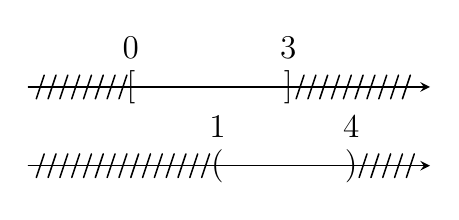
\begin{tikzpicture}[scale=1,line width=0.55pt, font={\fontsize{12pt}{0pt}}, line join=round, line cap=round, >=stealth]
		\begin{scope}
			\foreach \x in {1,2,3,...,8}
			{\draw (-1.3+\x*0.15+0.05,0.15)--(-1.3+\x*0.15-0.05,-0.15);}
			\foreach \x in {1,2,3,...,8,9,10}
			{\draw (2+\x*0.15+0.05,0.15)--(2+\x*0.15-0.05,-0.15);}
			\draw (0,0) node {$[$};
			\draw (0,0) node[yshift=0.5cm] {$0$};
			\draw (2,0) node[yshift=0.5cm] {$3$};
			\draw (2,0) node {$]$};
			\draw[->] (-1.3,0)--(3.8,0);
		\end{scope}
		\begin{scope}[yshift=-1cm]
			\foreach \x in {1,2,3,...,15}
			{\draw (-1.3+\x*0.15+0.05,0.15)--(-1.3+\x*0.15-0.05,-0.15);}
			\foreach \x in {1,2,3,...,5}
			{\draw (2.8+\x*0.15+0.05,0.15)--(2.8+\x*0.15-0.05,-0.15);}
			\draw (1.1,0) node {$($};
			\draw (1.1,0) node[yshift=0.5cm] {$1$};
			\draw (2.8,0) node[yshift=0.5cm] {$4$};
			\draw (2.8,0) node {$)$};
			\draw[->] (-1.3,0)--(3.8,0);
		\end{scope}
		\end{tikzpicture}
	\end{center}
	}
\end{ex}

%%==========Câu 19
\begin{ex}%[0D1K3-1]
Cho các tập hợp $A=\left\{x \in \mathbb{R} \mid x^2-9 \geq 0\right\} ; B=(0 ; 3)$. Biết $A \cup B=(-\infty ; a] \cup(b ;+\infty)$ Tính giá trị của biểu thức $a+b$.
	\choice
 {$a+b=0$}
 {\True $a+b=-3$}
{$a+b=3$}
{$a+b=6$}
\loigiai{Ta có $x^2-9 \geq 0 \Leftrightarrow \hoac{
		& x \leq-3 \\
		& x \geq 3 \\
	}$.\\
	Do đó $A=(-\infty ;-3] \cup[3 ;+\infty)$ Khi đó $A \cup B=(-\infty ;-3] \cup(0 ;+\infty)$.\\
	Suy ra $a=-3 ; b=0$. Vậy $a+b=-3$.
	}
\end{ex}

%%==========Câu 20
\begin{ex}%[0D1K3-2]
Cho hai tập hợp $A=\{n \in \mathbb{N} \mid n \leq 3\}$ và $B=\{x \in \mathbb{Z} \| x \mid<5\}$. Xác định $C_B A$.
\choice
{$C_B A=\{-4 ;-3 ;-2 ;-1\}$}
{$C_B A=\{-5 ;-4 ;-3 ;-2 ;-1 ; 4 ; 5\}$}
{\True $C_B A=\{-4 ;-3 ;-2 ;-1 ; 4\}$}
{$C_B A=\{-4 ;-3 ;-2 ;-1 ; 0\}$}
	\loigiai{Ta có $A=\{0 ; 1 ; 2 ; 3\}, B=\{-4 ;-3 ;-2 ;-1 ; 0 ; 1 ; 2 ; 3 ; 4\}$.\\
	 Suy ra $C_B A=B \backslash A=\{-4 ;-3 ;-2 ;-1 ; 4\}$.
	}
\end{ex}

%%==========Câu 21
\begin{ex}%[0D2B2-2]
	Miền tam giác $A B C$ kể cả ba cạnh sau đây là miền nghiệm của hệ bất phương trình nào trong bốn hệ bất phương trình dưới đây?
	\begin{center}
		\begin{tikzpicture}[scale=0.8,thick,>=stealth']
			\fill[thin,pattern=north east lines] (-1,3.5) -- (4,3.5) -- (4,-1.2) -- (-1,2.8) -- cycle;
			\fill[thin,pattern=north east lines] (-0.4,-3) -- (91/41,10/41) -- (4,-1.2) -- (4,-3) -- cycle;
			\fill[thin,pattern=north east lines] (-1,2.8) -- (0,2) -- (0,-3) -- (-0.4,-3) --(-1,-3) -- cycle;
			\draw[->] (-1,0) -- (4,0)node[above right]{$x$};
			\foreach \x in {1,2,3}
			\draw[shift={(\x,0)},color=black] (0pt,2pt) -- (0pt,-2pt) node[below] {\small $\x$};
			\draw[->,color=black] (0,-3) -- (0,3.5)node[above right]{$y$};
			\node[below right] at (0,0){$O$};
			\clip(-1,-3) rectangle (4,3.5);
			\draw[line width=1.2pt,smooth,samples=100,domain=-1:4] plot(\x,{5/4*(\x)-10/4});
				\draw[line width=1.2pt,smooth,samples=100,domain=-1:4] plot(\x,{10/5-4/5*(\x)});
				\foreach \y in {1,2,3}
				\draw[shift={(0,\y)},color=black] (2pt,0pt) -- (-2pt,0pt) node[left]{\small $\y$};
				\path 
				(0,2) coordinate (A)
				(90/41,10/41) coordinate (B)
				(0,-2.5) coordinate (C)
				;
					\foreach \x/\g in {A/60,B/90,C/-10}
				\draw[fill=black] (\x) circle (.036)+(\g:.35)
				node{$\x$};	
		\end{tikzpicture}
	\end{center}
	\choice
	{$\heva{
			& y \geq 0 \\
			& 5 x-4 y \geq 10 \\
			& 5 x+4 y \leq 10
		}$}
	{$\heva{
			& x>0 \\
			& 5 x-4 y \leq 10 \\
			& 4 x+5 y \leq 10
		}$} 
	{$\heva{
			& x \geq 0 \\
			& 4 x-5 y \leq 10 \\
			& 5 x+4 y \leq 10
		}$}
	{\True $\heva{
			& x \geq 0 \\
			& 5 x-4 y \leq 10 \\
			& 4 x+5 y \leq 10
		}$}
	\loigiai{Cạnh $A C$ có phương trình $x=0$ và cạnh $A C$ nằm trong miền nghiệm nên $x \geq 0$ là một bất phương trình của hệ.\\
	Cạnh $A B$ qua hai điểm $\left(\dfrac{5}{2} ; 0\right)$ và $(0 ; 2)$ nên có phương trình: $\dfrac{x}{\dfrac{5}{2}}+\dfrac{y}{2}=1 \Leftrightarrow 4 x+5 y=10$.\\
		Vậy hệ bất phương trình cần tìm là $\heva{
			& x \geq 0 \\
			& 5 x-4 y \leq 10 \\
			& 4 x+5 y \leq 10
		}$.
	}
\end{ex}

%%==========Câu 22
\begin{ex}%[0D1K2-2]
Trong các khẳng định sau khẳng định nào \textbf{đúng}?
\choice
{$\mathbb{R} \backslash \mathbb{Q}=\mathbb{N}$}
{$\mathbb{N}^* \cup \mathbb{N}=\mathbb{Z}$}
{$\mathbb{N}^* \cap \mathbb{Z}=\mathbb{Z}$}
{\True $\mathbb{N}^* \cap \mathbb{Q}=\mathbb{N}^*$}  
	\loigiai{Ta có $\mathbb{N}^* \subset \mathbb{Q} \Rightarrow \mathbb{N}^* \cap \mathbb{Q}=\mathbb{N}^*$. Nên chọn $\mathrm{D}$
	}
\end{ex}

%%==========Câu 23
\begin{ex}%[0D2K2-2]
Miền nghiệm (phần tô màu) của hệ bất phương trình $\heva{
	& x-2 y \geq 2 \\
	& 3 x+y>1 \\
	& x-y \geq 0
}$ trên mặt phẳng tọa độ là hình nào trong các hình dưới đây?
\begin{center}
\begin{tikzpicture}[scale=0.8,thick,>=stealth']
	\path 
	(0.25,0.25) coordinate (A)
	(4/7,-5/7) coordinate (B)
	(-2,-2) coordinate (C)
	;
	\fill[thin,pattern=north east lines] (-0.85,3.5) -- (A) -- (3.5,3.5) -- cycle;
	\fill[thin,pattern=north east lines] (A) -- (3.5,3.5) -- (3.5,-3) -- (1.3,-3)-- (B) -- cycle;
	\fill[thin,pattern=north east lines] (B)--(1.3,-3)--(-3,-3)--(-3,-2.5)--cycle;
	\fill[thin,pattern=north east lines] (-0.85,3.5)--(A)--(C)--(-3,-2.5)--(-3,3.5)--cycle;
	\draw[->] (-3,0) -- (3.5,0)node[above right]{$x$};
	
	\draw[->,color=black] (0,-3) -- (0,3.5)node[above right]{$y$};
	\node[above left] at (0,0){$O$};
	\draw (-2,3) node {\small$3x+y=1$};
	\draw (2,3) node {\small$x-y=0$};
	\draw (2.25,0.9) node {\small$x-2y=2$};
	\clip(-3,-4.1) rectangle (3.5,3.5);
	\draw[line width=1.2pt,smooth,samples=100,domain=-3:1.3] plot(\x,{-3*(\x)+1});
	\draw[line width=1.2pt,smooth,samples=100,domain=-3:4] plot(\x,{1/2*(\x)-1});
	\draw[line width=1.2pt,smooth,samples=100,domain=-3:4] plot(\x,{(\x)});
	\foreach \y in {1,2,3}
	\draw[shift={(0,\y)},color=black] (2pt,0pt) -- (-2pt,0pt) node[left]{\small $\y$};
	\draw (0.5,-3.5) node {\textit{Hình 1}};
%	\foreach \x/\g in {A/60,B/90,C/-10}
%	\draw[fill=black] (\x) circle (.036)+(\g:.35)
%	node{$\x$};	
\end{tikzpicture}~~~~~~~~~~~\begin{tikzpicture}[scale=0.8,thick,>=stealth']
\path 
(0.25,0.25) coordinate (A)
(4/7,-5/7) coordinate (B)
(-2,-2) coordinate (C)
;
\fill[thin,pattern=north east lines] (A)--(B)--(C)--cycle;
\draw[->] (-3,0) -- (3.5,0)node[above right]{$x$};

\draw[->,color=black] (0,-3) -- (0,3.5)node[above right]{$y$};
\node[above left] at (0,0){$O$};
\draw (-2,3) node {\small$3x+y=1$};
\draw (2,3) node {\small$x-y=0$};
\draw (2.25,0.9) node {\small$x-2y=2$};
\clip(-3,-4.1) rectangle (3.5,3.5);
\draw[line width=1.2pt,smooth,samples=100,domain=-3:1.3] plot(\x,{-3*(\x)+1});
\draw[line width=1.2pt,smooth,samples=100,domain=-3:4] plot(\x,{1/2*(\x)-1});
\draw[line width=1.2pt,smooth,samples=100,domain=-3:4] plot(\x,{(\x)});
\foreach \y in {1,2,3}
\draw[shift={(0,\y)},color=black] (2pt,0pt) -- (-2pt,0pt) node[left]{\small $\y$};
\draw (0.5,-3.5) node {\textit{Hình 2}};
%	\foreach \x/\g in {A/60,B/90,C/-10}
%	\draw[fill=black] (\x) circle (.036)+(\g:.35)
%	node{$\x$};	
\end{tikzpicture}\\
\begin{tikzpicture}[scale=0.8,thick,>=stealth']
\path 
(0.25,0.25) coordinate (A)
(4/7,-5/7) coordinate (B)
(-2,-2) coordinate (C)
;

\fill[thin,pattern=north east lines] (B)--(1.3,-3)--(-3,-3)--(3.5,-3)--(3.5,0.75)--cycle;

\draw[->] (-3,0) -- (3.5,0)node[above right]{$x$};

\draw[->,color=black] (0,-3) -- (0,3.5)node[above right]{$y$};
\node[above left] at (0,0){$O$};
\draw (-2,3) node {\small$3x+y=1$};
\draw (2,3) node {\small$x-y=0$};
\draw (2.25,0.9) node {\small$x-2y=2$};
\clip(-3,-4.1) rectangle (3.5,3.5);
\draw[line width=1.2pt,smooth,samples=100,domain=-3:1.3] plot(\x,{-3*(\x)+1});
\draw[line width=1.2pt,smooth,samples=100,domain=-3:4] plot(\x,{1/2*(\x)-1});
\draw[line width=1.2pt,smooth,samples=100,domain=-3:4] plot(\x,{(\x)});
\foreach \y in {1,2,3}
\draw[shift={(0,\y)},color=black] (2pt,0pt) -- (-2pt,0pt) node[left]{\small $\y$};
\draw (0.5,-3.5) node {\textit{Hình 3}};
%	\foreach \x/\g in {A/60,B/90,C/-10}
%	\draw[fill=black] (\x) circle (.036)+(\g:.35)
%	node{$\x$};	
\end{tikzpicture}~~~~~~~~~~~~\begin{tikzpicture}[scale=0.8,thick,>=stealth']
\path 
(0.25,0.25) coordinate (A)
(4/7,-5/7) coordinate (B)
(-2,-2) coordinate (C)
;

\fill[thin,pattern=north east lines] (C)--(-3,-3)--(-3,-2.5)--cycle;
\draw[->] (-3,0) -- (3.5,0)node[above right]{$x$};

\draw[->,color=black] (0,-3) -- (0,3.5)node[above right]{$y$};
\node[above left] at (0,0){$O$};
\draw (-2,3) node {\small$3x+y=1$};
\draw (2,3) node {\small$x-y=0$};
\draw (2.25,0.9) node {\small$x-2y=2$};
\clip(-3,-4.1) rectangle (3.5,3.5);
\draw[line width=1.2pt,smooth,samples=100,domain=-3:1.3] plot(\x,{-3*(\x)+1});
\draw[line width=1.2pt,smooth,samples=100,domain=-3:4] plot(\x,{1/2*(\x)-1});
\draw[line width=1.2pt,smooth,samples=100,domain=-3:4] plot(\x,{(\x)});
\foreach \y in {1,2,3}
\draw[shift={(0,\y)},color=black] (2pt,0pt) -- (-2pt,0pt) node[left]{\small $\y$};
\draw (0.5,-3.5) node {\textit{Hình 4}};
%	\foreach \x/\g in {A/60,B/90,C/-10}
%	\draw[fill=black] (\x) circle (.036)+(\g:.35)
%	node{$\x$};	
\end{tikzpicture}
\end{center}
	\choice
	{\textit{Hình 1}}
	{\textit{Hình 2}}
	{\True \textit{Hình 3}}
	{\textit{Hình 4}}  
	\loigiai{\textbf{Bước 1.} Xác định miền nghiệm của bất phương trình $x-2 y \geq 2$.
		\begin{itemize}
			\item Vẽ đường thẳng $d: x-2 y=2$.
			\item Vì $0-2.0=0<2$ nên tọa độ điểm $O(0 ; 0)$ không thỏa mãn bất phương trình $x-2 y \geq 2$.
		\end{itemize}
		Do đó, miền nghiệm của bất phương trình $x-2 y \geq 2$ là nửa mặt phẳng bờ là đường thẳng $x-2 y=2$ không chứa gốc tọa độ $O$.\\
		\textbf{Bước 2.} Tương tự, miền nghiệm của bất phương trình $3 x+y>1$ là nửa mặt phẳng bờ là đường thẳng $3 x+y=1$ không chứa gốc tọa độ $O$.\\
		\textbf{Bước 3.} Tương tự, miền nghiệm của bất phương trình $x-y \geq 0$ là nửa mặt phẳng bờ là đường thẳng $x-y=0$ chứa điểm $(1 ; 0)$.\\
		Khi đó, miền tô màu chính là giao các miền nghiệm của các bất phương trình trong hệ. Vậy miền nghiệm của hệ là miền tô màu.
	}
\end{ex}

%%==========Câu 24	
\begin{ex}%[0H1K1-2]
Cho góc $\alpha \in\left(90^{\circ} ; 180^{\circ}\right)$. Biết rằng $\sin \alpha=\dfrac{1}{3}$. Tính giá trị của $\cos \alpha$.
\choice
{$\cos \alpha=\dfrac{2}{3}$}
 {$\cos \alpha=\dfrac{ \pm 2 \sqrt{2}}{3}$}
 {$\cos \alpha=\dfrac{2 \sqrt{2}}{3}$}
{\True $\cos \alpha=\dfrac{-2 \sqrt{2}}{3}$}
 
	\loigiai{Ta có $\sin ^2 \alpha+\cos ^2 \alpha=1 \Rightarrow \cos ^2 \alpha=1-\sin ^2 \alpha=\dfrac{8}{9}$.\\
	Vì $\alpha \in\left(90^{\circ} ; 180^{\circ}\right) \Rightarrow \cos \alpha<0$.
		Nên $\cos \alpha=\dfrac{-2 \sqrt{2}}{3}$.
	}
\end{ex}

%%==========Câu 25
\begin{ex}%[0H1K2-2]
Cho tam giác $A B C$ có $A B=4, A C=6, A=120^{\circ}$. Độ dài cạnh $B C$ bằng
\choice
{$2 \sqrt{7}$}
{$8$}
{\True $2 \sqrt{19}$}
{$2 \sqrt{10}$}
\loigiai{Áp dụng định lí cosin trong tam giác $A B C$, ta có:
		$$
		B C^2=A B^2+A C^2-2 \cdot A B \cdot A C \cdot \cos A=4^2+6^2-2 \cdot 4 \cdot 6 \cdot \cos 120^{\circ}=76 \Rightarrow B C=\sqrt{76}=2 \sqrt{19}
		$$
	}
\end{ex}

%%==========Câu 26
\begin{ex}%[0H1K2-2]
Cho $\triangle M N P$ có độ dài cạnh và góc như hình vẽ bên dưới. Độ dài cạnh $M N$ có kết quả xấp xỉ bằng
\begin{center}	
	\begin{tikzpicture}[scale=1,line width=0.55pt, font={\fontsize{12pt}{0pt}}, line join=round, line cap=round, >=stealth]
		% Khai bao diem		
		\path
		(0,0) coordinate (M)
		(4,0) coordinate (P)
		(2.5,3) coordinate (N)
		;
		
		\draw ($(M)!1/2!(P)$) node[below] {\small$27$};
		\draw (M) node[yshift=0.2cm,xshift=0.5cm] {\small$43^\circ$};
		\draw (P) node[yshift=0.2cm,xshift=-0.5cm] {\small$69^\circ$};
		\draw (M)--(N)--(P)--(M);
		% vẽ điểm
		\foreach \x/\g in {M/-90,P/-90,N/90}
		\draw[fill=black] (\x) circle (.036)+(\g:.35)
		node{$\x$};	
		
	\end{tikzpicture}
\end{center}
\choice
{$26{,}8$}
{\True $27{,}2$}
{$27{,}6$}
{$24{,}4$}
\loigiai{Xét tam giác $M N P$ ta có:
	$$
	\widehat{M N P}=180^{\circ}-43^{\circ}-69^{\circ}=68^{\circ}
	$$
	$$
	\dfrac{M P}{\sin \widehat{M N P}}=\dfrac{M N}{\sin \widehat{M P N}} \text { ( định lý sin) }
	$$
	hay $\dfrac{27}{\sin 68^{\circ}}=\dfrac{M N}{\sin 69^{\circ}}$, khi đó $M N=\dfrac{27 \cdot \sin 69^{\circ}}{\sin 68^{\circ}} \approx 27,2$
	}
\end{ex}

%%==========Câu 27
\begin{ex}%[0H1K3-2]
Trượt Zipline là một trò chơi đang rất được ưa chuộng, đặc biệt là với giới trẻ và những người yêu thích sự mạo hiểm. Để chơi trượt zipline, người ta sẽ buộc một sợi dây cáp dài được nối từ một điểm có vị trí cao hơn và nối xuống một vị trí thấp hơn (thường dây cáp sẽ được nối vào đỉnh núi, thân núi hoặc một cột thép cao nhân tạo xuống). Một dây cáp zipline được nối từ một tháp cao $28$ feet (ft) xuống một chòi nghỉ có độ cao $11~(\mathrm{ft})$ so với mặt đất. Góc tạo bởi dây cáp lúc căng và cột thép là $85^{\circ}$ (xem hình vẽ). Tính chiều dài của dây cáp lúc được căng và không có người trượt trên đó. Với quy ước $1(\mathrm{ft})=0,3 (\mathrm{m})$, làm tròn kết quả đến chữ số thập phân thứ nhất.
\begin{center}
	\includegraphics[width=10cm]{image/0-GK1-CanhDieu-De6-NH23-24-H1}
\end{center}
	\choice
	{$96{,}4$}
	{$134{,}2$}
	{$37{,}9$}
	{\True$58{,}5$}
	\loigiai{
	\begin{center}	
		\begin{tikzpicture}[scale=1,line width=0.55pt, font={\fontsize{12pt}{0pt}}, line join=round, line cap=round, >=stealth]
			% Khai bao diem
			\draw (-1.5,0)--(5.5,0);		
			\path
			(-0.5,0) coordinate (D)
			(-0.5,1.75) coordinate (B)
			(-0.5,4) coordinate (A)
			(4.5,0) coordinate (E)
			(4.5,1.75) coordinate (C)
			;
				\draw (A) node[yshift=-0.5cm,xshift=0.4cm] {\small$85^\circ$};
			\draw (D)--(A)--(C)--(E) (B)--(C);
			\draw [<->] (-0.65,0)--(-0.65,1.75);
			\draw [<->] (-1.5,0)--(-1.5,4);
			\draw ($(-1.5,0)!1/2!(-1.5,4)$) node [xshift=-0.6cm] {\small$28~(\mathrm{ft})$};
			\draw ($(-0.65,0)!1/2!(-0.65,1.75)$) node [xshift=-0.6cm] {\small$11(\mathrm{ft})$};
			\draw ($(4.65,0)!1/2!(4.65,1.75)$) node [xshift=0.6cm] {\small$11(\mathrm{ft})$};
			\draw [<->] (4.65,0)--(4.65,1.75);
			\draw ($(D)!1/2!(E)$) node [above] {\small Mặt đất};
			% vẽ điểm
			\foreach \x/\g in {D/-90,B/180,A/180,C/0,E/-90}
			\draw[fill=black] (\x) circle (.036)+(\g:.35)
			node{$\x$};	
			
		\end{tikzpicture}
	\end{center}
	Mô phỏng lại như trên hình vẽ. Ta cần tính độ dài của đoạn thẳng $A C$\\
		Ta có $B D=C E=11 ~(\mathrm{ft}) \Rightarrow A B=A D-B D=28-11=17~(\mathrm{ft})$\\
		Xét tam giác $A B C$, ta có:
		$$
		\cos 85^{\circ}=\dfrac{A B}{A C} \Rightarrow A C=\dfrac{A B}{\cos 85^{\circ}}=\dfrac{17}{\cos 85^{\circ}}~(\mathrm{ft})=\dfrac{17}{\cos 85^{\circ}} \cdot 0,3=58{,}5~(\mathrm{m})
		$$
	}
\end{ex}

%%==========Câu 28
\begin{ex}%[0H1K2-2]
Cho tam giác $A B C$ biết $A B=50$, $B C=70$, $A=30^{\circ}$. Tính gần đúng diện tích tam giác $A B C$.
\choice
{$1583{,}56$}
{$1385{,}56$}
{$1538{,}56$}
{\True $1358{,}56$}
	\loigiai{
	Áp dụng định lý sin, ta có: $\dfrac{B C}{\sin A}=\dfrac{A B}{\sin C} \Rightarrow \sin C=\dfrac{50 \cdot \sin 30^{\circ}}{70}=\dfrac{5}{14}$
	$$
	\Rightarrow\left[\begin{array}{l}
		C \approx 20^{\circ} 55^{\prime} 30^{\prime \prime} \\
		C \approx 159^{\circ} 4^{\prime} 30^{\prime \prime}~(\text{loại})
	\end{array}\right.
	$$
	Nên $\widehat{B}=180^{\circ}-(\widehat{A}+\widehat{C}) \approx 129^{\circ} 4^{\prime} 30^{\prime \prime}$\\
	Áp dụng công thức diện tích, ta có: $S=\dfrac{1}{2} A B \cdot B C \cdot \sin B=\dfrac{1}{2} \cdot 50 \cdot 70 \cdot \sin \left(129^{\circ} 4^{\prime} 30 "\right) \approx 1358,56$.
	}
\end{ex}

%%==========Câu 29
\begin{ex}%[0D1G3-3]
Khảo sát phong trào tập luyện thể thao của một nhóm sinh viên, ta được 28 sinh viên chơi môn chạy bộ, 27 sinh viên chơi môn cầu lông, 25 sinh viên chơi môn bóng đá, 10 sinh viên chơi cả hai môn chạy bộ và cầu lông, 8 sinh viên chơi cả hai môn chạy bộ và bóng đá, 9 sinh viên chơi cả hai môn cầu lông và bóng đá, 3 sinh viên chơi cả ba môn chạy bộ, cầu lông và bóng đá. Số sinh viên chơi ít nhất một môn thể thao (chạy bộ, cầu lông, bóng đá) là
\choice
{$54$}
{$57$}
{$55$}
{\True $56$}
	\loigiai{
\begin{center}	
	\begin{tikzpicture}[scale=1,line width=0.55pt, font={\fontsize{12pt}{0pt}}, line join=round, line cap=round, >=stealth]
		% Khai bao diem		
		\draw (2,0) arc[start angle=0,end angle=360,x radius=2.5cm,y radius =1.5cm] ;
		\draw (-4,0) node {\textbf{Chạy bộ}};
		\draw (4.5,0) arc[start angle=0,end angle=360,x radius=2.5cm,y radius =1.5cm] ;
		\draw (5.5,0) node {\textbf{Cầu lông}};
		\draw (0.8,-1.5) circle (1.8cm);
		\draw (3.3,-2.75) node {\textbf{Bóng đá}};
		\draw 
		(-2,0) node {$13$}
		(0.75,0.7) node {$7$}
		(0.75,-0.5) node {$3$}
		(-0.5,-0.95) node {$5$}
		(2,-0.95) node {$6$}
		(0.5,-2) node {$11$}
		(3,0) node {$11$}
		;
	\end{tikzpicture}
\end{center}		
Ta dùng biểu đồ Ven để giải.\\
Từ biểu đồ Ven ta có số sinh viên chơi ít nhất một môn thể thao là $$13+7+3+5+11+6+11=56~(\text{học sinh})$$
	}
\end{ex}

%%==========Câu 30
\begin{ex}%[0H1K1-2]
Cho tam giác $A B C$ có $B C=a$, $C A=b$, $A B=c$ thỏa mãn $\dfrac{a+b}{6}=\dfrac{b+c}{5}=\dfrac{c+a}{7}$. Giá trị của biểu thức $P=\cos A+2 \cos B+4 \cos C$ bằng
	\choice
{$-\dfrac{15}{4}$}
{ $\dfrac{15}{4}$}
{$-\dfrac{17}{4}$}
{\True $\dfrac{17}{4}$}
	\loigiai{
	Đặt $\dfrac{a+b}{6}=\dfrac{b+c}{5}=\dfrac{c+a}{7}=t \Rightarrow \heva{
		& a+b=6 t \\
		& b+c=5 t \\
		& c+a=7 t
	}\Rightarrow a+b+c=9 t$ và $\heva{
	& a=4 t \\
	& b=2 t  \\
	& c=3 t
	}$.\\
	Áp dụng hệ quả định lí Côsin, ta có:\\
	$\cos A=\dfrac{b^2+c^2-a^2}{2 \cdot b \cdot c}=\dfrac{4 t^2+9 t^2-16 t^2}{2 \cdot 2 t \cdot 3 t}=-\dfrac{1}{4}$ \\
	$\cos B=\dfrac{c^2+a^2-b^2}{2 \cdot c \cdot a}=\dfrac{9 t^2+16 t^2-4 t^2}{2.3 t \cdot 4 t}=\dfrac{7}{8}$\\
	$\cos C=\dfrac{a^2+b^2-c^2}{2 \cdot a \cdot b}=\dfrac{16 t^2+4 t^2-9 t^2}{2 \cdot 4 t \cdot 2 t}=\dfrac{11}{16}$\\
	Vậy $P=\cos A+2 \cos B+4 \cos C=\dfrac{17}{4}$.
	}
\end{ex}

%%==========Câu 31
\begin{ex}%[0H2G2-2]
Cho tam giác $A B C$ có trọng tâm $G$ và diện tích bằng $10~(\mathrm{cm}^2)$. Gọi $O$ là tâm đường tròn ngoại tiếp tam giác $A B C$. Gọi $M, N, P$ lần lượt là hình chiếu của $G$ trên các cạnh $B C, C A, A B$. Biết $O A=4~(\mathrm{cm})$, $G O=3 ~(\mathrm{cm})$. Diện tích tam giác $M N P$ bằng
\choice
{$\dfrac{35}{8}~(\mathrm{cm}^2)$}
{$\dfrac{35}{2} ~(\mathrm{cm}^2)$}
{\True $\dfrac{35}{32}~(\mathrm{cm}^2)$}
{$\dfrac{125}{32}~(\mathrm{cm}^2)$}
	\loigiai{
		\begin{center}	
			\begin{tikzpicture}[scale=1,line width=0.55pt, font={\fontsize{12pt}{0pt}}, line join=round, line cap=round, >=stealth]
				% Khai bao diem	
				\def\r{2.5}	
				\path
				(0,0) coordinate (O)
				(-\r,0) coordinate (X)
				($(O)!\r cm!20:(X)$) coordinate (B)
				($(O)!\r cm!180-20:(X)$) coordinate (C)
				($(O)!\r cm!-73:(X)$) coordinate (A)
				($(A)!(B)!(C)$) coordinate (Y)
				($(B)!(A)!(C)$) coordinate (Z)
				($(B)!1/2!(C)$) coordinate (T)
				($(A)!2/3!(T)$) coordinate (G)
				($(A)!(G)!(B)$) coordinate (P)
				($(A)!(G)!(C)$) coordinate (N)
				($(C)!(G)!(B)$) coordinate (M)
				;
				\draw pic[draw,thin,angle radius=2.5mm] {right angle = A--Z--B};
				\draw pic[draw,thin,angle radius=2.5mm] {right angle = B--Y--A};
				\draw pic[draw,thin,angle radius=2.5mm] {right angle = G--M--B};
				\draw pic[draw,thin,angle radius=2.5mm] {right angle = G--P--A};
				\draw pic[draw,thin,angle radius=2.5mm] {right angle = G--N--C};
				\draw (A)--(B)--(C)--(A)--(Z) (B)--(Y) (P)--(G)--(M) (N)--(G) (M)--(N)--(P)--(M) (A)--(T);
				% vẽ điểm
				\foreach \x/\g in {A/90,B/-90,C/-90,M/-90,N/45,P/140,O/0,G/77}
				\draw[fill=black] (\x) circle (.036)+(\g:.35)
				node{$\x$};	
				
			\end{tikzpicture}
		\end{center}
	$\bullet$ Kí hiệu $a, b, c$ lần lượt là 3 cạnh $B C, A C, A B$ của tam giác $A B C$;\\
	$h_a, h_b$ lần lượt là đường cao xuất phát từ đỉnh $A, B$;\\
	$m_a, m_b, m_c$ lần lượt là 3 đường trung tuyến xuất phát từ đỉnh $A, B, C$.\\
	$\bullet$ Ta có $S_{\triangle M N P}=S_{\triangle G M N}+S_{\triangle G M P}+S_{\triangle G N P}$ và $S_{\triangle G M N}=\dfrac{1}{2} \cdot G M \cdot G N \cdot \sin \left(180^{\circ}-C\right)=\dfrac{h_a h_b \sin C}{18}$\\
	Lại có $h_a=\dfrac{2 S_{\triangle A B C}}{a}=\dfrac{20}{a} ; h_b=\dfrac{20}{b}$ và $\sin C=\dfrac{c}{2 R}=\dfrac{c}{8}$.\\
	Suy ra $S_{\triangle G M N}=\dfrac{h_a h_b \sin C}{18}=\dfrac{20 \cdot 20 \cdot c}{18.8 a b}=\dfrac{25 c^2}{9 a b c}$.\\
	Mà $S_{\triangle A B C}=\dfrac{a b c}{4 R} \Rightarrow 10=\dfrac{a b c}{4.4} \Rightarrow a b c=160 \Rightarrow S_{\triangle G M N}=\dfrac{25 c^2}{9 a b c}=\dfrac{25 c^2}{9.160}=\dfrac{5 c^2}{288}$.\\
	Tương tự, $S_{\triangle G N P}=\dfrac{5 a^2}{288} ; S_{\triangle G P M}=\dfrac{5 b^2}{288}$.\\
	Suy ra $S_{\triangle M N P}=S_{\triangle G M N}+S_{\triangle G M P}+S_{\triangle G N P}=\dfrac{5\left(a^2+b^2+c^2\right)}{288}$\quad\quad(1)\\
	% $\bullet$ Mặt khác, $\overrightarrow{O A}^2+\overrightarrow{O B}^2+\overrightarrow{O C}^2=(\overrightarrow{G A}-\overrightarrow{G O})^2+(\overrightarrow{G B}-\overrightarrow{G O})^2+(\overrightarrow{G C}-\overrightarrow{G O})^2$
	% $$
	% \begin{aligned}
	% 	& =\overrightarrow{G A}^2+\overrightarrow{G B}^2+\overrightarrow{G C}^2-2 \overrightarrow{G O}(\overrightarrow{G A}+\overrightarrow{G B}+\overrightarrow{G C})+3 \overrightarrow{G O}^2 \\
	% 	& =G A^2+G B^2+G C^2+3 G O^2
	% \end{aligned}
	% $$
	$\bullet$ Ta có công thức $3R^2=GA^2+GB^2+GC^2+3GO^2$ (chứng minh sử dụng tổng vector).\\
	Suy ra $3 \cdot 4^2=G A^2+G B^2+G C^2+3.3^2 \Rightarrow G A^2+G B^2+G C^2=21$\quad(2)\\
	$\bullet$ Lại có $G A^2+G B^2+G C^2=\dfrac{4}{9}\left(m_a^2+m_b^2+m_c^2\right)$
	$$
	\begin{aligned}
		& \Leftrightarrow G A^2+G B^2+G C^2=\dfrac{4}{9}\left[\dfrac{2\left(b^2+c^2\right)-a^2}{4}+\dfrac{2\left(a^2+c^2\right)-b^2}{4}+\dfrac{2\left(a^2+b^2\right)-c^2}{4}\right] \\
		& \Leftrightarrow G A^2+G B^2+G C^2=\dfrac{a^2+b^2+c^2}{3}\quad(3)
	\end{aligned}
	$$
	Từ (2) và (3) suy ra $21=\dfrac{a^2+b^2+c^2}{3} \Leftrightarrow a^2+b^2+c^2=63$\quad(4)\\
	Thay (4) vào (3) ta có $S_{\triangle M N P}=\dfrac{5.63}{288}=\dfrac{35}{32} \mathrm{~cm}^2$.
	}
\end{ex}

%%==========Câu 32
\begin{ex}%[0H1G3-2]
Hai bạn An và Hưng cùng xuất phát từ điểm $P$, đi theo hai hướng khác nhau và tạo với nhau một góc $40^{\circ}$ để đến đích là điểm $D$. Biết rằng họ dừng lại để ăn trưa lần lượt tại $A$ và $B$ (\textit{như hình vẽ}). Hỏi Hưng phải đi bao xa nữa để đến được đích?
\begin{center}	
	\begin{tikzpicture}[scale=1,line width=0.55pt, font={\fontsize{12pt}{0pt}}, line join=round, line cap=round, >=stealth]
		% Khai bao diem		
		\path
		(0,0) coordinate (P)
		(5,0) coordinate (B)
		($(P)!5cm!40:(B)$) coordinate (A)
		($(A)!2cm!100:(P)$) coordinate (D)
		;
		\draw pic[draw,angle radius=5.56mm] {angle = B--P--A};
		\draw (P) node [yshift=0.25cm,xshift=0.9cm] {\small$40^\circ$};
		\draw pic[draw,angle radius=5mm] {angle = P--A--D};
		\draw (A) node [yshift=-0.7cm] {\small$100^\circ$};
		\draw ($(A)!1/2!(P)$) node [xshift=-0.6cm] {\small$8~\mathrm{km}$};
		\draw ($(A)!1/2!(D)$) node [xshift=0.4cm,yshift=0.2cm] {\small$3~\mathrm{km}$};
		\draw ($(B)!1/2!(P)$) node [yshift=0.2cm] {\small$7~\mathrm{km}$};
		\draw (P)--(B)--(D)--(A)--(P);
		% vẽ điểm
		\foreach \x/\g in {A/90,P/180,B/0,D/0}
		\draw[fill=black] (\x) circle (.036)+(\g:.35)
		node{$\x$};	
		
	\end{tikzpicture}
\end{center}
	\choice
	{$3{,}352~(\mathrm{km})$}
	{\True $3{,}516~(\mathrm{km})$}
	{$4{,}125~(\mathrm{km})$}
	{$2{,}563~(\mathrm{km})$}
	\loigiai{
	\begin{center}	
		\begin{tikzpicture}[scale=1,line width=0.55pt, font={\fontsize{12pt}{0pt}}, line join=round, line cap=round, >=stealth]
			% Khai bao diem		
			\path
			(0,0) coordinate (P)
			(5,0) coordinate (B)
			($(P)!5cm!40:(B)$) coordinate (A)
			($(A)!2cm!100:(P)$) coordinate (D)
			;
			\draw pic[draw,angle radius=5.56mm] {angle = B--P--A};
			\draw (P) node [yshift=0.25cm,xshift=0.9cm] {\small$40^\circ$};
			\draw pic[draw,angle radius=5mm] {angle = P--A--D};
			\draw (A) node [yshift=-0.7cm] {\small$100^\circ$};
			\draw ($(A)!1/2!(P)$) node [xshift=-0.6cm] {\small$8~\mathrm{km}$};
			\draw ($(A)!1/2!(D)$) node [xshift=0.4cm,yshift=0.2cm] {\small$3~\mathrm{km}$};
			\draw ($(B)!1/2!(P)$) node [yshift=0.2cm] {\small$7~\mathrm{km}$};
			\draw (P)--(B)--(D)--(A)--(P)--(D);
			% vẽ điểm
			\foreach \x/\g in {A/90,P/180,B/0,D/0}
			\draw[fill=black] (\x) circle (.036)+(\g:.35)
			node{$\x$};	
			
		\end{tikzpicture}
	\end{center}
	Ta có: $P D=\sqrt{A P^2+A D^2-2 A P \cdot A D \cdot \cos P A D}=\sqrt{8^2+3^2-2 \cdot 8 \cdot 3 \cdot \cos 100^{\circ}} \approx 9,0186 \mathrm{~km}$.\\
	Do đó: $\dfrac{P D}{\sin \widehat{P A D}}=\dfrac{A D}{\sin \widehat{A P D}} \Rightarrow \sin \widehat{A P D}=\dfrac{A D \cdot \sin \widehat{P A D}}{P D}=\dfrac{3 \cdot \sin 100^{\circ}}{9,0186} \approx 0,3276$\\
	$\Rightarrow \widehat{A P D} \approx 19,1232^{\circ}$
	$$
	\begin{aligned}
		& \Rightarrow D P B=40^{\circ}-19,27^{\circ}=20,8768^{\circ} . \\
		& \Rightarrow B D=\sqrt{P D^2+P B^2-2 P D \cdot P B \cdot \cos D P B}=\sqrt{9,0186^2+7^2-2 \cdot 9,0186 \cdot 7 \cdot \cos 20,8768^{\circ}} \\
		& \Rightarrow B D \approx 3,516 \mathrm{~km} .
	\end{aligned}
	$$
	Vậy Brett phải đi thêm $3{,}516$ km.
	}
\end{ex}

%%==========Câu 33
\begin{ex}%[0D1G3-1]
Cho hai tập hợp $A=(-1;2]$ và $B=\left\{x \in \mathbb{R}\,|\, mx \geq 1\right\}$ $(\text{với } m \text{ là tham số thực})$. Xác định tất cả giá trị của tham số $m$ để $A \cap B =\varnothing$.
	\choice
	{\True $m \in \left[-1;\dfrac{1}{2}\right)$}
	{ $m \in (-\infty;-1] \cup \left[0;\dfrac{1}{2}\right)$}
	{$m \in \left[-1;\dfrac{1}{2}\right) \backslash \{0\}$}
	{$m \in \left[-1;\dfrac{1}{2}\right]$}
	\loigiai{
	Ta xét ba trường hợp
	\begin{itemize}
		\item Nếu $m=0$ suy ra $B=\varnothing$ do đó $A \cap B=\varnothing$ nên $m=0$ thỏa mãn yêu cầu bài toán.
		\item Nếu $m>0$, từ $m x \geq 1 \Leftrightarrow x \geq \dfrac{1}{m}$ hay $B=\left[\dfrac{1}{m} ;+\infty\right)$, do đó để $A \cap B=\varnothing$ thì $2<\dfrac{1}{m}$
		$\Leftrightarrow m<\dfrac{1}{2}$. Do đó $0<m<\dfrac{1}{2}$ thỏa mãn yêu cầu bài toán.
		\item Nếu $m<0$, từ $m x \geq 1 \Leftrightarrow x \leq \dfrac{1}{m}$ hay $B=\left(-\infty ; \dfrac{1}{m}\right)$, do đó để $A \cap B=\varnothing$ thì $\dfrac{1}{m} \leq-1$\\
		$\Leftrightarrow m \geq-1$. Do đó $-1 \leq m<0$ thỏa mãn yêu cầu bài toán.
	\end{itemize}
	Vậy $-1 \leq m < \dfrac{1}{2}$ thỏa mãn yêu cầu bài toán.
	}
\end{ex}


%%==========Câu 34
\begin{ex}%[0H1K2-2]
Cho tam giác $A B C$ có góc $C$ nhọn, $A H$ và $B K$ là hai đường cao, $H K=\sqrt{7}$, diện tích tứ giác $A B H K$ bằng $7$ lần diện tích tam giác $C H K$. Khi đó bán kính đường tròn ngoại tiếp tam giác $A B C$ bằng
\choice
 {\True $4$} 
 {$7$} 
{$8$} 
{$\sqrt{14}$}
	\loigiai{
	Ta có $S_{A B H K}=7 S_{C H K} \Rightarrow S_{A B C}=8 S_{C H K} \cdot \dfrac{S_{A B C}}{S_{C H K}}=\dfrac{\dfrac{1}{2} C A \cdot C B \cdot \sin C}{\dfrac{1}{2} C K \cdot C H \cdot \sin C}=\dfrac{C A \cdot C B}{C K \cdot C H}=8$\quad(1)\\
	$\triangle A H C$ vuông tại $H$, ta có $\cos C=\dfrac{C H}{C A}$\quad (2)\\
	$\triangle B K C$ vuông tại $K$, ta có $\cos C=\dfrac{C K}{C B}$\quad (3)\\
	Từ (1), (2), (3) ta có $\cos ^2 C=\dfrac{1}{8}$.\\
	Ta có $\triangle H C K$ đồng dạng với $\triangle A C B\ (c-g-c)$\\
	$$\Rightarrow \dfrac{H K}{A B}=\dfrac{C H}{A C}=\cos C=\dfrac{1}{2 \sqrt{2}}
	\Rightarrow A B=2 \sqrt{2} H K=2 \sqrt{14}$$
	Bán kính đường tròn ngoại tiếp tam giác $A B C$ là:
	$$
	R=\dfrac{A B}{2 \sin C}=\dfrac{A B}{2 \sqrt{1-\cos ^2 C}}=\dfrac{2 \sqrt{14}}{2 \sqrt{1-\dfrac{1}{8}}}=4
	$$
	}
\end{ex}

%%==========Câu 35
\begin{ex}%[0D1G3-2]
Cho các tập hợp $A=(-\infty ; m)$ và $B=[3 m-1 ; 3 m+2]$. Có bao nhiêu giá trị nguyên $m \in[-2022 ; 2022]$ để $A \subset C_{\mathbb{R}} B$.
	\choice
{$2020$} 
{\True $2022$} 
 {$2019$}
 {$2021$} 
	\loigiai{
	Ta có $C_{\mathbb{R}} B=(-\infty ; 3 m-1) \cup(3 m+2 ;+\infty)$.\\
	Suy ra $A \subset C_{\mathbb{R}} B \Leftrightarrow m \leq 3 m-1 \Leftrightarrow m \geq \dfrac{1}{2}$.\\
	Mà $m \in[-2022 ; 2022]$ và $m \in \mathbb{Z}$ nên có 2022 giá trị $m$ thỏa đề.
	}
\end{ex}



\noindent{\bf\fontfamily{qag}\selectfont\color{violet}B. PHẦN TỰ LUẬN}


%%==========Bài 1
\begin{bt}%[0D1K3-2]
Cho tập hợp $A=\{a, b, c, d\} ; B=\{b ; d ; e\} ; C=\{a ; b ; c\}$ Chứng minh: $$A \cap(B \backslash C)=(A \cap B) \backslash(A \cap C).$$
	\loigiai{
Ta có $B \backslash C=\{d ; e\} \Rightarrow A \cap(B \backslash C)=\{d\}$
$$
A \cap B=\{b ; d\}, A \cap C=\{a ; b ; c\} \Rightarrow(A \cap B) \backslash(A \cap C)=\{d\}
$$
Vậy $A \cap(B \backslash C)=(A \cap B) \backslash(A \cap C)$
	}
\end{bt}

%%==========Bài 2
\begin{bt}%[0H1K3-2]
Cho tam giác $A B C$ có $A B=3~(\mathrm{cm})$, $A C=5~(\mathrm{cm})$,  $\widehat{A}=60^{\circ}$. Hãy tính:
\begin{enumerate}
	\item Độ dài cạnh $B C$ và số đo $\widehat{ABC}$ và $\widehat{ACB}$ (làm tròn đến phút).
	\item Diện tích tam giác $A B C$.
\end{enumerate}
	\loigiai{
	\begin{enumerate}
		\item +) Áp dụng định lý cos trong $\triangle A B C$ ta có:
		$$
		\begin{aligned}
			& B C^2=A B^2+A C^2-2 A B \cdot A C \cdot \cos A=3^2+5^2-2 \cdot 3 \cdot 5 \cdot \cos 60^{\circ}=19 \\
			& \Rightarrow B C=\sqrt{19} \mathrm{~cm} .
		\end{aligned}
		$$
		+) Áp dụng định lý Sin trong $\triangle A B C$ ta có:
		$$
		\begin{aligned}
			& \dfrac{B C}{\sin A}=\dfrac{A C}{\sin B} \Leftrightarrow \sin B=\dfrac{A C \cdot \sin A}{B C}=\dfrac{5 \cdot \sin 60^{\circ}}{\sqrt{19}}=\dfrac{5 \sqrt{57}}{38} \\
			& \Rightarrow B \approx 83^{\circ} 25^{\prime} \\
			& \Rightarrow C=180^{\circ}-(A+B) \approx 180^{\circ}-\left(60^{\circ}+83^{\circ} 25^{\prime}\right)=36^{\circ} 35^{\prime} .
		\end{aligned}
		$$
		\item Diện tích tam giác $A B C$ là:
		$$
		S_{\triangle A B C}=\dfrac{1}{2} A B \cdot A C \cdot \sin A=\dfrac{1}{2} \cdot 3 \cdot 5 \cdot \sin 60^{\circ}=\dfrac{15 \sqrt{3}}{14}\left(\mathrm{cm}^2\right) .
		$$
	\end{enumerate}
	}
\end{bt}

%%==========Bài 3
\begin{bt}%[0D2G2-3]
Một người ăn kiêng muốn trộn hai loại thức ăn $A$ và $B$, để tạo ra một hỗn hợp chứa ít nhất $50 \mathrm{~g}$ protein, ít nhất $130 \mathrm{mg}$ canxi và không quá 550 calo. Giá trị dinh dưỡng của thức ăn loại $A$ và loại $B$ được cho trong bảng sau:\\
\centerline{\begin{tabular}{|c|c|c|c|}
	\hline Thức ăn & Protein (g/ly) & Canxi (mg/ly) & Calo (ly) \\
	\hline$A$ & 20 & 20 & 100 \\
	\hline$B$ & 10 & 50 & 150 \\
	\hline
\end{tabular}}\\
Biết rằng giá tiền một ly thức ăn loại $A$ là 120.000 đồng, một ly thức ăn loại $B$ là 50.000 đồng. Hỏi người ăn kiêng phải sử dụng bao nhiêu ly thức ăn mỗi loại để số tiền bỏ ra là ít nhất.
	\loigiai{
	\begin{center}
		\begin{tikzpicture}[scale=0.8,thick,>=stealth']
			\path 
			(1,3) coordinate (A)
			(1.5,2) coordinate (B)
			(4,1) coordinate (C)
			;
			\draw [thin, gray!40, step=1.0cm] (-2,-1.5) grid (5,4.6);
			\fill[thin,pattern=north east lines] (A)--(B)--(C)--cycle;
			\draw[->] (-2,0) -- (5,0)node[above right]{$x$};
			
			\draw[->,color=black] (0,-1.5) -- (0,4.6)node[above right]{$y$};
			\node[above left] at (0,0){$O$};
			
			\clip(-2,-1.5) rectangle (5,4.6);
			\draw[line width=1.2pt,smooth,samples=100,domain=-2:4.7] plot(\x,{-2/5*(\x)+13/5});
			\draw[line width=1.2pt,smooth,samples=100,domain=-3:4.7] plot(\x,{-2*(\x)+5});
			\draw[line width=1.2pt,smooth,samples=100,domain=-3:4.7] plot(\x,{-2/3*(\x)+11/3});
			\foreach \y in {1,2,3}
			\draw[shift={(0,\y)},color=black] (2pt,0pt) -- (-2pt,0pt) node[left]{\small $\y$};
			\draw (0.5,-3.5) node {\textit{Hình 1}};
				\foreach \x/\g in {A/60,B/-140,C/90}
				\draw[fill=black] (\x) circle (.036)+(\g:.35)
				node{$\x$};	
		\end{tikzpicture}
	\end{center}
	Gọi $x, y$ lần lượt là số ly thức ăn loại $A$ và loại $B$ người ăn kiêng sử dụng.\\
	Số tiền người ăn kiêng bỏ ra: $f(x, y)=120000 x+50000 y$ (đồng)\\
	Từ giả thiết của bài toán ta viết lại bằng hệ bất phương trình sau đây:
	$$
	\left\{\begin{array} { l } 
		{ 2 0 x + 1 0 y \geq 5 0 } \\
		{ 2 0 x + 5 0 y \geq 1 3 0 } \\
		{ 1 0 0 x + 1 5 0 y \leq 5 5 0 }
	\end{array} \Leftrightarrow \left\{\begin{array}{l}
		2 x+y \geq 5 \\
		2 x+5 y \geq 13 \\
		2 x+3 y \leq 11
	\end{array}\right.\right.
	$$
	Ta biểu diễn miền nghiệm của hệ bất phương trình trên như sau:\\
	Miền nghiệm của hệ bất phương trình trên là miền trong của tam giác $A B C$, kể cả 3 cạnh của tam giác đó.\\
	Ta có: $A(1 ; 3), B\left(\dfrac{3}{2} ; 2\right), C(4 ; 1)$.\\
	Ta có: $f(1 ; 3)=270000$ đồng; $f\left(\dfrac{3}{2} ; 2\right)=280000$ đồng; $f(4 ; 1)=530000$ đồng.\\
	Vậy người ăn kiêng phải sử dụng 1 ly thức ăn loại $A$ và 3 ly thức ăn loại $B$.
	}
\end{bt}

%%==========Bài 4
\begin{bt}%[0H1K3-1]
Cho hình chữ nhật $A B C D$ có $A D=a,(a>0)$, điểm $M$ là trung điểm đoạn $A B$ và $\sin \widehat{M D B}=\dfrac{1}{3}$. Tính độ dài đoạn $A B$ theo $a$.
	\loigiai{
		\begin{center}	
			\begin{tikzpicture}[scale=1,line width=0.55pt, font={\fontsize{12pt}{0pt}}, line join=round, line cap=round, >=stealth]
				% Khai bao diem		
				\path
				(0,0) coordinate (D)
				(0,2) coordinate (A)
				(2*3,0) coordinate (C)
				($(A)+(C)-(D)$) coordinate (B)
				($(A)!1/2!(B)$) coordinate (M)
				;
				
				\draw (A)--(B)--(C)--(D)--(A) (D)--(M) (D)--(B);
				% vẽ điểm
				\foreach \x/\g in {A/90,B/90,C/-90,D/-90,M/90}
				\draw[fill=black] (\x) circle (.036)+(\g:.35)
				node{$\x$};	
				
			\end{tikzpicture}
		\end{center}
	Đặt $A B=x(x>0)$, khi đó $A M=M B=\dfrac{x}{2}$.\\
	Do $0^{\circ}<M D B<90^{\circ}$ nên $\cos M D B>0$, do đó $\cos M D B=\sqrt{1-\sin ^2 M D B}=\sqrt{1-\dfrac{1}{9}}=\dfrac{2 \sqrt{2}}{3}$.\\
	Ta có $D M=\sqrt{A D^2+A M^2}=\sqrt{a^2+\dfrac{x^2}{4}}$ và $B D=\sqrt{A D^2+A B^2}=\sqrt{a^2+x^2}$.\\
	Áp dụng định lí Cosin trong tam giác $M B D$ ta có
	$$
	\begin{aligned}
		& M B^2=D M^2+D B^2-2 D M \cdot D B \cos \widehat{M D B} \\
		\Leftrightarrow & \dfrac{x^2}{4}=a^2+\dfrac{x^2}{4}+a^2+x^2-2 \cdot \sqrt{a^2+\dfrac{x^2}{4}} \cdot \sqrt{a^2+x^2} \cdot \dfrac{2 \sqrt{2}}{3} \\
		\Leftrightarrow & \dfrac{4 \sqrt{2}}{3} \cdot \sqrt{\left(a^2+\dfrac{x^2}{4}\right)\left(a^2+x^2\right)}=2 a^2+x^2 \\
		\Leftrightarrow & x^4-4 a^2 x^2+4 a^4=0 \Leftrightarrow x=a \sqrt{2} .
	\end{aligned}
	$$
	Vậy $A B=a \sqrt{2}$.
	}
\end{bt}

\Closesolutionfile{ans}
\inputans{10}{ans/ans-0-GK1-CTST-De6-NH23-24}